\section{}
\begin{figure}[H]
  \centering
\includegraphics[page=40, width=\textwidth]{../../notes/Ch8_W20_TCP_IP.pdf}
\end{figure}

On the server side, it starts in the CLOSED state, which means there is no
connection. When the server performs a passive open, it creates a transmission
control block and readies itself to recieve a SYN segment. This is known as the
LISTEN state.
An active opener sends the server a SYN segment. The server responds
with its own SYN segment. The server also
acknowledges the client’s SYN by sending a ACK.
This is known as the SYN+RCVD state.
When the server
receives the ACK from the client in response to the SYN it sent, the
connection is established. (The ESTABLISHED state)

\begin{figure}[H]
  \centering
\includegraphics[page=41, width=\textwidth]{../../notes/Ch8_W20_TCP_IP.pdf}
\end{figure}
On the client side, when the server decides to terminate the connection, it
receives a FIN. The client's application also sends a FIN segment. Once the
client has sent its FIN, it transitions to the FIN\_WAIT\_1 state. In the normal
case, it receives an ACK from the server for the FIN which was sent, and goes to
the FIN\_WAIT\_2 state where it continues to wait for the FIN segment from the
server. When it does, it sends an ACK for the server and transitions to the
TIME\_WAIT state. From there, the client waits for double the maximum segment
lifetimes to make sure the ACK sent to the server was received. When the timer
expires, the connection is terminated and the state CLOSED is reached.

What can also happen is that in the FIN\_WAIT\_1 state, the client receives the
server's FIN segment before it acknowledges the client’s FIN segment. The client
sends an ACK to let the server it received the FIN segment, and the transition
is made to the CLOSING state. From there, the client waits for double the
maximum segment lifetimes to make sure the ACK sent to the server was received.
When the timer expires, the connection is terminated and the state CLOSED is
reached.

